La IA se está volviendo más móvil de lo que solía ser, ya que los dispositivos más 
pequeños se están empaquetando con más potencia computacional. Los dispositivos móviles, que simplemente se usaban para hacer llamadas telefónicas y enviar mensajes de texto, ahora se han transformado en teléfonos inteligentes con la introducción de la IA. Estos dispositivos ahora son capaces de aprovechar el poder cada vez mayor de la inteligencia artificial para aprender el comportamiento y las preferencias del usuario, mejorar las fotografías, llevar a cabo conversaciones completas y mucho más. Se espera que las capacidades de un teléfono inteligente con inteligencia artificial solo crezcan día a día. Según Gartner, para 2022, el $80\%$ de los teléfonos inteligentes estarán habilitados para IA.

Huawei ha lanzado el Kirin 970 SoC, que permite experiencias de IA en el dispositivo utilizando una unidad de procesamiento de red neuronal especialmente dedicada. Los dispositivos de Apple están equipados con un chip de inteligencia artificial llamado motor neuronal, que es parte del chip A11 Bionic. Está dedicado al aprendizaje automático y las tareas de aprendizaje profundo, como el reconocimiento facial y de voz, la grabación de animojis y la detección de objetos mientras se captura una imagen. Qualcomm y MediaTek han lanzado sus propios chips que permiten soluciones de inteligencia artificial en el dispositivo. Exynos 9810, anunciado por Samsung, es un chip que se basa en redes neuronales como Snapdragon 845 de Qualcomm. Los dispositivos Samsung 2018, Galaxy S9 y S9 +, incluyeron estos chips según el país donde se comercializan. Con su Galaxy S9, la compañía dejó bastante claro que integraría IA para mejorar el funcionamiento de la cámara del dispositivo y la traducción de texto en tiempo real. La última serie Samsung Galaxy S10 funciona con Qualcomm Snapdragon 855 para admitir cálculos de IA en el dispositivo.

Google Translate Word Lens y el asistente personal de Bixby se han utilizado para desarrollar la función. Con las tecnologías implementadas, es posible que el dispositivo traduzca hasta 54 idiomas. Los teléfonos, que son lo suficientemente inteligentes como para decidir entre un sensor de f / 2.4 yf / 1.5, son muy adecuados para capturar fotografías en condiciones de poca luz. Google Pixel 2 aprovecha el poder del aprendizaje automático para integrar ocho unidades de procesamiento de imágenes utilizando su coprocesador, Pixel Visual Core.

\section{Chips de IA}

La incorporación de chips de IA no solo ha ayudado a lograr una mayor eficiencia y potencia computacional, sino que también ha preservado los datos y la privacidad del usuario. Las ventajas de incluir chips de IA en dispositivos móviles se pueden enumerar de la siguiente manera:

\begin{itemize}
\item Rendimiento.- las CPU de los dispositivos móviles en la fecha actual no son adecuadas para las demandas del aprendizaje automático. Los intentos de implementar modelos de aprendizaje automático en estos dispositivos a menudo dan como resultado un servicio lento y un agotamiento más rápido de la batería, lo que genera una mala experiencia del usuario. Esto se debe a que las CPU carecen de la eficiencia para hacer enormes cantidades de pequeños cálculos como lo requieren los cálculos de IA. Los chips de inteligencia artificial, algo similares a los chips de unidades de procesamiento gráfico (GPU) que son responsables de manejar gráficos en los dispositivos, brindan un espacio separado para realizar cálculos relacionados exclusivamente con el aprendizaje automático y los procesos de aprendizaje profundo. Esto permite que la CPU concentre su tiempo en otras tareas importantes. Con la incorporación de hardware de inteligencia artificial especializado, el rendimiento y la duración de la batería de los dispositivos han mejorado.
\item Privacidad del usuario.- el hardware también garantiza una mayor seguridad de la privacidad y la seguridad del usuario. En los dispositivos móviles tradicionales, los procesos de análisis de datos y aprendizaje automático requerirían el envío de fragmentos de los datos del usuario a la nube, lo que representa una amenaza para la privacidad de los datos del usuario y la seguridad de los dispositivos móviles. Con los chips de IA en el dispositivo en acción, todos los análisis y cálculos necesarios se pueden realizar sin conexión en el propio dispositivo. Esta incorporación de hardware dedicado en dispositivos móviles ha reducido enormemente los riesgos de que los datos de un usuario sean pirateados o filtrados.
\item Eficiencia.- en el mundo real, tareas como el reconocimiento y el procesamiento de imágenes podrían ser mucho más rápidas con la incorporación de chips de IA. La unidad de procesamiento de redes neuronales de Huawei es un ejemplo muy adecuado aquí. Puede reconocer imágenes con una eficiencia de 2000 imágenes por segundo. La compañía afirma que esto es 20 veces más rápido que el tiempo que toma una CPU estándar. Cuando trabaja con números de punto flotante de 16 bits, puede realizar 1,92 teraflops o 1 billón de operaciones flotantes por segundo. El motor neuronal de Apple puede manejar alrededor de 600 mil millones de operaciones por segundo.
\item Economía.- los chips de IA en el dispositivo reducen la necesidad de enviar datos a la nube. Esta capacidad permite a los usuarios acceder a los servicios sin conexión y guardar datos. Por lo tanto, las personas que utilizan las aplicaciones se salvan de pagar por los servidores. Esto es ventajoso tanto para los usuarios como para los desarrolladores.
\end{itemize}


\section{Experiencia de usuario mejorada con IA en dispositivos móviles}

El uso de IA ha mejorado enormemente la experiencia del usuario en dispositivos móviles. Esto se puede clasificar ampliamente en las siguientes categorías.

\section{Personalización}

La personalización significa principalmente modificar un servicio o un producto para que se adapte a las preferencias de un individuo específico, a veces relacionado con grupos de individuos. En los dispositivos móviles, el uso de IA ayuda a mejorar la experiencia del usuario al hacer que el dispositivo y las aplicaciones se adapten a los hábitos del usuario y a su perfil único en lugar de aplicaciones genéricas orientadas al perfil. Los algoritmos de inteligencia artificial en los dispositivos móviles aprovechan los datos específicos del usuario disponibles, como la ubicación, el historial de compras y los patrones de comportamiento, para predecir y personalizar las interacciones presentes y futuras, como la actividad preferida del usuario o la música durante un momento particular del día.

Por ejemplo, AI recopila datos sobre el historial de compras del usuario y los compila con los demás datos que se obtienen del tráfico en línea, dispositivos móviles, sensores integrados en dispositivos electrónicos y vehículos. Estos datos compilados se utilizan luego para analizar el comportamiento del usuario y permitir que las marcas tomen las acciones necesarias para mejorar la tasa de participación del usuario. Por lo tanto, los usuarios pueden aprovechar los beneficios de las aplicaciones con inteligencia artificial para obtener resultados personalizados, lo que reducirá su tiempo de desplazamiento y les permitirá explorar más productos y servicios.

Los mejores ejemplos son los sistemas de recomendación que se ejecutan a través de plataformas de compras como Walmart, Amazon o plataformas de medios como YouTube o Netflix.

\section{Asistentes virtuales}

Un asistente virtual es una aplicación que comprende los comandos de voz y completa tareas para el usuario. Son capaces de interpretar el habla humana utilizando Natural Language Understanding (NLU) y generalmente responden a través de voces sintetizadas. Puede usar un asistente virtual para casi todas las tareas que un asistente personal real haría por usted, es decir, hacer llamadas a personas en su nombre, tomar notas que dicte, encender o apagar las luces de su hogar / oficina con la ayuda de la automatización del hogar, reproducir música para usted o incluso simplemente hablar con usted sobre cualquier tema del que le gustaría hablar. Un asistente virtual podría recibir comandos en forma de texto, audio o gestos visuales. Los asistentes virtuales se adaptan a los hábitos de los usuarios con el tiempo y se vuelven más inteligentes.

Aprovechando el poder de la PNL, un asistente virtual puede reconocer comandos del lenguaje hablado e identificar personas y mascotas a partir de imágenes que subes a tu asistente o guardas en cualquier álbum en línea al que tengan acceso.

Los asistentes virtuales más populares en el mercado en este momento son Alexa de Amazon, Google Assistant, Siri de iPhone, Cortana de Microsoft y Bixby que se ejecutan en dispositivos Samsung. Algunos de los asistentes virtuales son oyentes pasivos y solo responden cuando reciben un comando de activación específico. Por ejemplo, el Asistente de Google se puede activar usando "Ok Google" o "OK Google", y luego se le puede ordenar que apague las luces usando "Apagar las luces de la habitación" o se puede usar para llamar a una persona de su lista de contactos usando "Hacer una llamada a <nombre del contacto>". En Google IO '18, Google presentó la IA de reserva de llamadas telefónicas dúplex, demostrando que el Asistente de Google no solo sería capaz de hacer una llamada, sino que también podría mantener una conversación y, potencialmente, reservar una reserva en una peluquería por sí solo. .

El uso de asistentes virtuales está creciendo exponencialmente y se espera que alcance los 1.800 millones de usuarios en 2021. El $54\%$ de los usuarios estuvo de acuerdo en que los asistentes virtuales ayudan a simplificar las tareas diarias y el $31\%$ ya usa asistentes en su vida diaria. Además, el $64\%$ de los usuarios aprovechan los asistentes virtuales para más de un propósito.


\section{Reconocimiento facial}

La tecnología que es lo suficientemente poderosa para identificar o verificar un rostro o comprender una expresión facial a partir de imágenes y videos digitales se conoce como reconocimiento facial. Este sistema generalmente funciona comparando los rasgos faciales más comunes y prominentes de una imagen dada con los rostros almacenados en una base de datos. El reconocimiento facial también tiene la capacidad de comprender patrones y variaciones basados en las texturas y la forma facial de un individuo para reconocer de manera única a una persona y, a menudo, se describe como una aplicación biométrica basada en IA.

Inicialmente, el reconocimiento facial era una forma de aplicación informática; sin embargo, recientemente, se está utilizando ampliamente en plataformas móviles. El reconocimiento facial, acompañado de datos biométricos como el reconocimiento de huellas dactilares e iris, encuentra una aplicación común en los sistemas de seguridad de los dispositivos móviles. Generalmente, el proceso de reconocimiento facial se realiza en dos pasos: la extracción y selección de características es el primero y la clasificación de objetos es el segundo. Desarrollos posteriores han introducido varios otros métodos, como el uso del algoritmo de reconocimiento facial, el reconocimiento tridimensional, el análisis de la textura de la piel y las cámaras térmicas.

Face ID, introducido en el iPhone X de Apple, es un sucesor de autenticación biométrica del sistema de autenticación basado en huellas dactilares que se encuentra en varios teléfonos inteligentes basados en Android. El sensor de reconocimiento facial de Face ID consta de dos partes: un módulo Romeo y un módulo Julieta. El módulo Romeo se encarga de proyectar más de 30.000 puntos infrarrojos en la cara del usuario. La contraparte de este módulo, el módulo Juliet, lee el patrón formado por los puntos en la cara del usuario. Luego, el patrón se envía a un módulo Secure Enclave en el dispositivo en la CPU del dispositivo para confirmar si la cara coincide con el propietario o no. Apple no puede acceder directamente a estos patrones faciales. El sistema no permite que la autorización funcione cuando los ojos del usuario están cerrados, lo cual es una capa adicional de seguridad.

La tecnología aprende de los cambios en la apariencia de un usuario y funciona con maquillaje, barbas, anteojos, lentes de sol y sombreros. También funciona en la oscuridad. El Flood Illuminator es un flash infrarrojo dedicado que proyecta luz infrarroja invisible en la cara del usuario para leer correctamente los puntos faciales y ayuda al sistema a funcionar en condiciones de poca luz o incluso en la oscuridad total. A diferencia de los iPhones, los dispositivos Samsung se basan principalmente en el reconocimiento facial bidimensional acompañado de un escáner de iris que funciona como reconocimiento biométrico en Galaxy Note 8. El principal vendedor de teléfonos inteligentes premium en India, OnePlus, también depende únicamente del reconocimiento facial bidimensional.

Se espera que el mercado global de software que se beneficia del reconocimiento facial crezca de $\$ 3,85$ mil millones de dólares en 2017 a $\$ 9,78$ mil millones de dólares en 2023. La región de Asia Pacífico, que posee alrededor del $16\%$ de su participación de mercado, es la región de más rápido crecimiento.

\section{Cámaras impulsadas por IA}

La integración de la IA en las cámaras les ha permitido reconocer, comprender y mejorar escenas y fotografías. Las cámaras AI pueden comprender y controlar los diversos parámetros de las cámaras. Estas cámaras funcionan según los principios de una técnica de procesamiento de imágenes digitales llamada fotografía computacional. Utiliza algoritmos en lugar de procesos ópticos que buscan utilizar la visión artificial para identificar y mejorar el contenido de una imagen. Estas cámaras utilizan modelos de aprendizaje profundo que se entrenan en un enorme conjunto de datos de imágenes, que comprende varios millones de muestras, para identificar automáticamente las escenas, la disponibilidad de luz y el ángulo de la escena que se captura.

Cuando la cámara apunta en la dirección correcta, los algoritmos de IA de la cámara se encargan de cambiar la configuración de la cámara para producir la mejor calidad de imagen. Bajo el capó, el sistema que permite la fotografía impulsada por IA no es simple. Los modelos utilizados están altamente optimizados para producir la configuración correcta de la cámara al detectar las características de la escena que se capturarán casi en tiempo real. También pueden agregar exposición dinámica, ajustes de color y el mejor efecto posible para la imagen. A veces, las imágenes pueden ser posprocesadas automáticamente por los modelos de IA en lugar de procesarse durante el clic de la fotografía para reducir la sobrecarga computacional del dispositivo.

Hoy en día, los dispositivos móviles generalmente están equipados con cámaras de doble lente. Estas cámaras usan dos lentes para agregar el efecto bokeh (que en japonés significa "desenfoque") en las fotografías. El efecto bokeh agrega un sentido borroso al fondo alrededor del sujeto principal, haciéndolo estéticamente agradable. Los algoritmos basados en IA ayudan a simular el efecto que identifica al sujeto y difumina la parte restante produciendo efectos de retrato.

La cámara Google Pixel 3 funciona en dos modos de disparo llamados Top Shot y Photobooth. Inicialmente, la cámara captura varios fotogramas antes y después del momento que el usuario intenta capturar. Los modelos de IA que están disponibles en el dispositivo pueden elegir el mejor marco. Esto es posible gracias a la gran cantidad de entrenamiento que se proporciona al sistema de reconocimiento de imágenes de la cámara, que luego puede seleccionar las imágenes más atractivas, casi como si un humano las estuviera recogiendo. El modo Photobooth permite al usuario simplemente sostener el dispositivo hacia una escena de acción, y las imágenes se toman automáticamente en el momento en que la cámara predice que será un momento perfecto.

\section{Texto predictivo}

El texto predictivo es una tecnología de entrada, generalmente utilizada en aplicaciones de mensajería, que sugiere palabras al usuario según las palabras y frases que se ingresan. La predicción que sigue a cada pulsación de tecla es única en lugar de producir una secuencia repetida de letras en el mismo orden constante. El texto predictivo puede permitir que se ingrese una palabra completa con una sola pulsación de tecla, lo que puede acelerar significativamente el proceso de entrada. Esto hace que las tareas de escritura de entrada, como escribir un mensaje de texto, escribir un correo electrónico o realizar una entrada en una libreta de direcciones, sean altamente eficientes con el uso de menos teclas del dispositivo. El sistema de texto predictivo vincula el estilo de interfaz preferido del usuario y su nivel de habilidad aprendida para operar el software de texto predictivo. El sistema eventualmente se vuelve más inteligente al analizar y adaptarse al idioma del usuario. El diccionario T9 es un buen ejemplo de tales predictores de texto. Analiza la frecuencia de las palabras utilizadas y da como resultado varias palabras más probables. También es capaz de considerar combinaciones de palabras.

Quick Type es una función de texto predictivo que fue anunciada por Apple en su versión iOS 8. Utiliza aprendizaje automático y PNL, lo que permite que el software cree diccionarios personalizados basados en los hábitos de escritura del usuario. Estos diccionarios se utilizan posteriormente para realizar predicciones. Estos sistemas de predicción también dependen del contexto de la conversación y son capaces de distinguir entre lenguajes formales e informales. Además, admite varios idiomas en todo el mundo, incluidos inglés de EE. UU., Inglés de Reino Unido, inglés de Canadá, inglés de Australia, francés, alemán, italiano, portugués de Brasil, español y tailandés.
Google también introdujo una nueva función que ayudaría a los usuarios a redactar y enviar correos electrónicos más rápido que antes. La función, llamada Redacción inteligente, comprende el texto escrito para que la IA pueda sugerir palabras y frases para terminar las oraciones. La función de redacción inteligente ayuda a los usuarios a ahorrar tiempo al escribir correos electrónicos al corregir errores ortográficos y gramaticales, además de sugerir las palabras que los usuarios escriben con más frecuencia. La respuesta inteligente es otra característica, similar a las sugerencias de respuesta en los mensajes de LinkedIn, que sugiere respuestas que se pueden enviar con un solo clic, de acuerdo con el contexto del correo electrónico recibido por el usuario. Por ejemplo, si el usuario recibe un correo electrónico felicitándolo por una solicitud aceptada, es probable que la función de respuesta inteligente brinde opciones para responder con: "¡Gracias!", "Gracias por avisarme" y "Gracias por aceptando mi solicitud ". Los usuarios pueden hacer clic en la respuesta preferida y enviar una respuesta rápida.

En la década de 1940, Lin Yutang creó una máquina de escribir en la que las teclas de accionamiento sugerían los caracteres que seguían a los seleccionados.

\section{Conceptos básicos del aprendizaje profundo}

En el año 1959, Arthur Samuel acuñó el término aprendizaje automático. En una suave reformulación de su definición de aprendizaje automático, el campo de la informática que permite a las máquinas aprender de experiencias pasadas y producir predicciones basadas en ellas cuando se les proporciona información desconocida se llama aprendizaje automático.

Se puede establecer una definición más precisa de aprendizaje automático de la siguiente manera:

Un programa de computadora que mejora su desempeño, P, en cualquier tarea, T, aprendiendo de su experiencia, E, con respecto a la tarea T, se llama programa de aprendizaje automático.
Usando la definición anterior, en una analogía que es común en este momento, T es una tarea relacionada con la predicción, mientras que P es la medida de precisión alcanzada por un programa de computadora mientras realiza la tarea, T, en base a lo que el programa pudo hacer. aprender, y el aprendizaje se llama E. Con el aumento de E, el programa de computadora hace mejores predicciones, lo que significa que P mejora porque el programa realiza la tarea T con mayor precisión.
En el mundo real, es posible que te encuentres con un profesor que enseña a un alumno a realizar una determinada tarea y luego evalúa la habilidad del alumno para realizar la tarea haciendo que el alumno rinda un examen. Cuanta más formación reciba el alumno, mejor podrá realizar la tarea y mejor será su puntuación en el examen.

\begin{thm}[Aprendizaje Profundo]
En informática, el aprendizaje profundo se refiere a un modelo de aprendizaje automático que tiene más de una capa de aprendizaje involucrada. Lo que esto significa es que el programa de computadora está compuesto por múltiples algoritmos a través de los cuales los datos pasan uno por uno para finalmente producir la salida deseada.
\end{thm}

Los sistemas de aprendizaje profundo se crean utilizando el concepto de redes neuronales. Las redes neuronales son composiciones de capas de neuronas conectadas entre sí de manera que los datos pasan de una capa de neuronas a otra hasta que llegan a la capa final o de salida. Cada capa de neuronas recibe la entrada de datos en una forma que puede o no ser la misma que la forma en que se proporcionaron inicialmente los datos como entrada a la red neuronal.

\begin{figure}[htb]
\centering
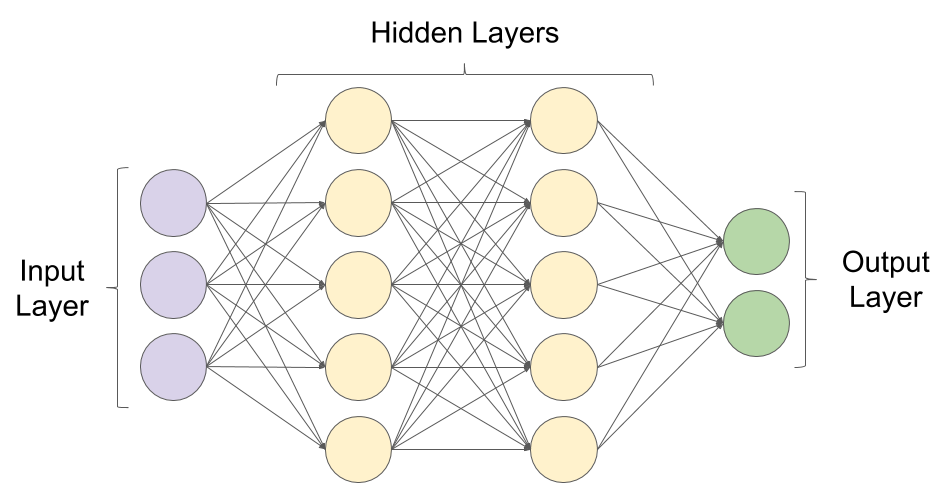
\includegraphics[width=0.7\textwidth]{capitulo1/red.png}
\caption{Estructura de una red neuronal}
\label{cap1:001}
\end{figure} 

\subsection{La capa de entrada}

La capa que contiene los valores de entrada se llama capa de entrada. Algunos argumentan que esta capa no es en realidad una capa, sino solo una variable que contiene los datos y, por lo tanto, son los datos en sí mismos, en lugar de ser una capa. Sin embargo, las dimensiones de la matriz que contiene la capa son importantes y deben definirse correctamente para que la red neuronal se comunique con la primera capa oculta; por lo tanto, es conceptualmente una capa que contiene datos.

\subsection{La capa oculta}


Cualquier capa que sea un intermediario entre la capa de entrada y la capa de salida se denomina capa oculta. Una red neuronal típica utilizada en entornos de producción puede contener cientos de capas de entrada. A menudo, las capas ocultas contienen una mayor cantidad de neuronas que la capa de entrada o la de salida. Sin embargo, en algunas circunstancias especiales, esto podría no ser cierto. Tener un mayor número de neuronas en las capas ocultas se suele hacer para procesar los datos en una dimensión distinta a la de entrada. Esto permite que el programa alcance información o patrones que pueden no ser visibles en los datos en el formato en el que están presentes cuando el usuario los introduce en la red.

La complejidad de una red neuronal depende directamente del número de capas de neuronas en la red. Si bien una red neuronal puede descubrir patrones más profundos en los datos al agregar más capas, también aumenta el costo computacional de la red. También es posible que la red pase a un estado erróneo llamado sobreajuste. Por el contrario, si la red es demasiado simple, o, en otras palabras, no es lo suficientemente profunda, llegará a otro estado erróneo llamado subadaptación.

\subsubsection{Sobreajuste y desajuste}

En los cursos de ciencia de datos, se explica que un modelo de sobreajuste tiene una alta varianza y un bajo sesgo en el conjunto de entrenamiento, lo que conduce a una mala generalización de los nuevos datos de prueba. Analicemos esa desconcertante definición en términos de nuestro intento de aprender inglés. El modelo que queremos construir es una representación de cómo comunicarse usando el idioma inglés. Nuestros datos de entrenamiento son las obras completas de Shakespeare y nuestro conjunto de pruebas es Nueva York. Si medimos el desempeño en términos de aceptación social, entonces nuestro modelo no se generaliza ni se traduce a los datos de prueba. Eso parece sencillo hasta ahora, pero ¿qué pasa con la varianza y el sesgo?
La varianza es cuánto cambia un modelo en respuesta a los datos de entrenamiento. Como simplemente estamos memorizando el conjunto de entrenamiento, nuestro modelo tiene una gran variación: depende en gran medida de los datos de entrenamiento. Si leemos las obras completas de J.K. Rowling en lugar de Shakespeare, el modelo será completamente diferente. Cuando se aplica un modelo con alta varianza en un nuevo conjunto de pruebas, no puede funcionar bien porque todo se pierde sin los datos de entrenamiento. Es como un estudiante que ha memorizado los problemas en el libro de texto, solo para sentirse indefenso cuando se enfrenta a problemas del mundo real.

El sesgo es la otra cara de la variación, ya que representa la fuerza de nuestras suposiciones que hacemos sobre nuestros datos. En nuestro intento de aprender inglés, nos formamos hipótesis, modelo iniciales, y confiamos en el trabajo del Bardo para enseñarnos todo sobre el idioma. Este bajo sesgo puede parecer positivo: ¿por qué querríamos estar sesgados hacia nuestros datos? Sin embargo, siempre debemos ser escépticos sobre la capacidad de los datos para contarnos la historia completa. Cualquier proceso natural genera ruido y no podemos estar seguros de que nuestros datos de entrenamiento capturen todo ese ruido. A menudo, debemos hacer algunas suposiciones iniciales sobre nuestros datos y dejar espacio en nuestro modelo para las fluctuaciones que no se ven en los datos de entrenamiento. Antes de comenzar a leer, deberíamos haber decidido que las obras de Shakespeare no podían literalmente enseñarnos inglés por sí mismas, lo que nos habría llevado a ser cautelosos a la hora de memorizar los datos de entrenamiento.
Para resumir hasta ahora: \textbf{el sesgo se refiere a cuánto ignoramos los datos, y la varianza se refiere a qué tan dependiente es nuestro modelo de los datos}. En cualquier modelo, siempre habrá una compensación entre el sesgo y la varianza y cuando construimos modelos, intentamos lograr el mejor equilibrio. El sesgo frente a la varianza es aplicable a cualquier modelo, desde el más simple hasta el más complejo, y es un concepto crítico de entender para los científicos de datos.

Vimos que un modelo que se adapta demasiado tiene una alta varianza y un sesgo bajo. ¿Qué pasa con lo contrario: baja varianza y alto sesgo? Esto se conoce como desajuste: en lugar de seguir los datos de entrenamiento demasiado de cerca, un modelo que no encaja ignora las lecciones de los datos de entrenamiento y no aprende la relación subyacente entre entradas y salidas.
Pensemos en esto en términos de nuestro ejemplo. Aprendiendo de nuestro intento anterior de construir un modelo de inglés, decidimos hacer algunas suposiciones sobre el modelo antes de tiempo. También cambiamos nuestros datos de entrenamiento y miramos todos los episodios del programa Friends para aprender inglés por nosotros mismos. Para evitar repetir nuestros errores desde el primer intento, asumimos de antemano que solo las oraciones que comienzan con las palabras más comunes del idioma (the, be, to, of y, a) son importantes. Cuando estudiamos, no prestamos atención a otras frases, confiando en que construiremos un modelo mejor.
Después de un largo período de formación, volvemos a salir a las calles de Nueva York. Esta vez nos va un poco mejor, pero de nuevo, nuestras conversaciones no van a ninguna parte y nos vemos obligados a admitir la derrota. Si bien sabemos algo de inglés y podemos comprender un número limitado de oraciones, no pudimos aprender la estructura fundamental del idioma debido a nuestro sesgo sobre los datos de entrenamiento. El modelo no sufre de una gran variación, ¡pero lo corregimos en exceso de nuestro intento inicial y no lo ajustamos!

\begin{figure}[htb]
\centering
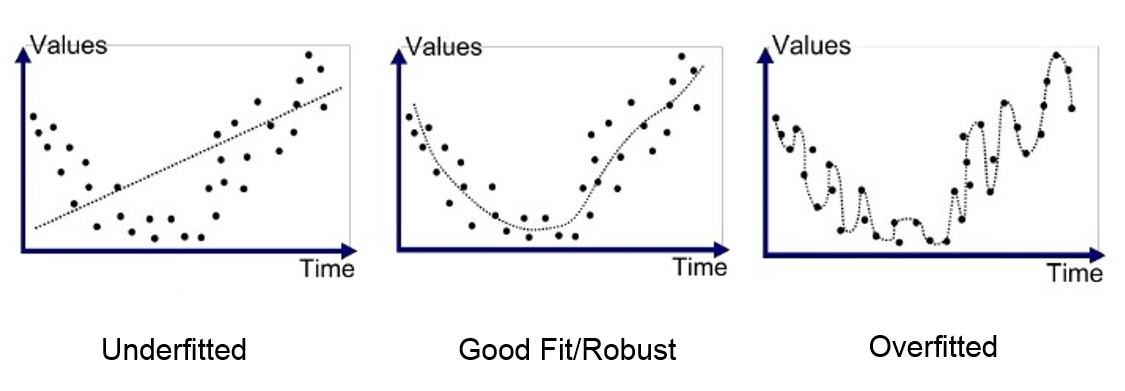
\includegraphics[width=0.7\textwidth]{capitulo1/sobreajuste.png}
\caption{Sobreajuste y subadaptación}
\label{cap1:002}
\end{figure} 

¿Qué podemos hacer? Prestamos estricta atención a los datos y sobreajustamos. Ignoramos los datos y encajamos. ¡Tiene que haber una manera de encontrar el equilibrio óptimo! Afortunadamente, existe una solución bien establecida en ciencia de datos llamada \textbf{validación}. En nuestro ejemplo, usamos solo un conjunto de entrenamiento y un conjunto de prueba. Esto significaba que no podíamos saber de antemano cómo funcionaría nuestro modelo en el mundo real. Idealmente, tendríamos un conjunto de "pruebas previas" para evaluar nuestro modelo y realizar mejoras antes de la prueba real. Esta "prueba previa" se conoce como un conjunto de validación y es una parte fundamental del desarrollo del modelo.
Nuestros dos fracasos para aprender inglés nos han hecho mucho más sabios y ahora decidimos utilizar un conjunto de validación. Usamos tanto el trabajo de Shakespeare como el programa Friends porque hemos aprendido más datos que casi siempre mejoran un modelo. La diferencia esta vez es que después del entrenamiento y antes de salir a la calle, evaluamos nuestro modelo en un grupo de amigos que se reúnen cada semana para discutir eventos actuales en inglés. La primera semana, casi nos echan de la conversación porque nuestro modelo del lenguaje es tan malo. Sin embargo, este es solo el conjunto de validación, y cada vez que cometemos errores podemos ajustar nuestro modelo. Eventualmente, podemos mantener nuestra conversación con el grupo y declarar que estamos listos para el conjunto de pruebas. Aventurándonos en el mundo real una vez más, ¡finalmente logramos el éxito! Nuestro modelo ahora es muy adecuado para la comunicación porque tenemos un elemento crucial, un conjunto de validación para el desarrollo y la optimización del modelo.

Este ejemplo está necesariamente simplificado. En los modelos de ciencia de datos, utilizamos numerosos conjuntos de validación porque, de lo contrario, terminamos sobreajustando el conjunto de validación. Esto se aborda mediante la validación cruzada, donde dividimos los datos de entrenamiento en diferentes subconjuntos, o podemos usar múltiples conjuntos de validación si tenemos muchos datos. Este ejemplo conceptual todavía cubre todos los aspectos del problema. Ahora, cuando escuche sobre sobreajuste frente a desajuste y sesgo frente a varianza, tendrá un marco conceptual para comprender el problema y cómo solucionarlo.

La ciencia de datos puede parecer compleja, pero en realidad se basa en una serie de bloques de construcción básicos. Algunos son:

\begin{itemize}

\item Sobreajuste: demasiada confianza en los datos de entrenamiento
\item Underfitting: una falla para aprender las relaciones en los datos de entrenamiento
\item Varianza alta: el modelo cambia significativamente en función de los datos de entrenamiento
\item Sesgo alto: las suposiciones sobre el modelo llevan a ignorar los datos de entrenamiento
\end{itemize}

El sobreajuste y el desajuste provocan una mala generalización en el conjunto de prueba
Un conjunto de validación para el ajuste del modelo puede evitar un ajuste insuficiente y excesivo.
La ciencia de datos y otros campos técnicos no deben separarse de nuestra vida cotidiana. Al explicar conceptos con ejemplos del mundo real, podemos ponerlos en contexto. Si entendemos el marco, entonces podemos completar los detalles utilizando las técnicas sobre problemas. La próxima publicación proporcionará un ejemplo usando gráficos y métricas, así que si quieres un respaldo más sólido, échale un vistazo.


\section{La capa de salida}

La capa final en la que se produce y almacena la salida deseada se llama capa de salida. Esta capa a menudo corresponde al número de categorías de salida deseadas o tiene una sola neurona que contiene la salida de regresión deseada.

\section{La función de activación}

La función de activación

Cada capa de la red neuronal se somete a la aplicación de una función llamada función de activación. Esta función desempeña el papel de mantener los datos contenidos dentro de las neuronas dentro de un rango normalizado, que de otro modo crecería demasiado o demasiado pequeño y conduciría a errores en el cálculo relacionados con el manejo de grandes coeficientes decimales o grandes números en computadoras. Además, es la función de activación la que permite a la red neuronal manejar la no linealidad de los patrones en los datos.

